\section{Vergleich der einzelnen Rahmenwerke}
%Multiplatform
%vergleich mit anderen frameworks
%Warum haben wir uns für Xamarin entschieden?
%- von VS2019 unterstützt
%- gratis, lizenzfrei
%- ...
%Welche Alternativen?
%- Native Programmierung
%- ...
%
\section{Build-Umgebung}
Aufgrund obiger Aufstellung wurde Visual Studio 2019 der Firma Microsoft als Entwicklungsumgebung gewählt.
Diese steht für Schüler und Private gratis auf der Seite {\href{https://visualstudio.microsoft.com/}{https://visualstudio.microsoft.com/}} zum Download zur Verfügung.
%versionsvergleich hier https://visualstudio.microsoft.com/vs/compare/
Visual Studio ist das offizielle Werkzeug für die Programmierung mit dem Xamarin-Rahmenwerk.

%Betriebssystem, Hardwareanforderungen
%
Die minimalen Hardware-Anforderungen können der \href{https://docs.microsoft.com/en-us/visualstudio/releases/2019/system-requirements}{Microsoft-Dokumentation des Visual Studio} entnommen werden:

\begin{itemize}
    \item Unterstützte Betriebssysteme
        \begin{itemize}
            \item Windows 10, Version 1703 oder höher: Home, Professional, Education und Enterprise (LTSC und S werden nicht unterstützt)
            \item Windows Server 2019: Standard und Datacenter
            \item Windows Server 2016: Standard und Datacenter
            \item Windows 8.1 (mit Update 2919355): Core, Professional und Enterprise
            \item Windows Server 2012 R2 (mit Update 2919355): Essentials, Standard, Datacenter
            \item Windows 7 SP1 (mit neuesten Windows-Updates): Home Premium, Professional, Enterprise, Ultimate
        \end{itemize}
    \item Hardware
        \begin{itemize}
            \item 1,8-GHz-Prozessor oder schneller; Quad-Core oder besser empfohlen
            \item 2 GB RAM; 8 GB RAM empfohlen (mindestens 2,5 GB bei Ausführung auf einem virtuellen Computer)
            \item Speicherplatz auf der Festplatte: Mindestens 800 MB, je nach installierten Features bis zu 210 GB des verfügbaren Speicherplatzes. Eine typische Installation erfordert 20–50 GB freien Speicherplatz.
            \item Festplattengeschwindigkeit: Zur Verbesserung der Leistung installieren Sie Windows und Visual Studio auf einem Festkörperlaufwerk (SSD).
            \item Grafikkarte, die eine Auflösung von mindestens 720p (1280 x 720) unterstützt. Visual Studio funktioniert am besten mit einer Auflösung von WXGA (1366 x 768) oder höher.
        \end{itemize}
\end{itemize}
%Quellenangabe!!
%Anforderungen für Android Emulator
% Der Android-Emulator hat zusätzliche Anforderungen, die über die grundlegenden Systemanforderungen für Android Studio hinausgehen, die im Folgenden beschrieben werden:

%     SDK-Tools 26.1.1 oder höher
%     64-Bit-Prozessor
%     Fenster: CPU mit UG-Unterstützung (uneingeschränkter Gast)
%     HAXM 6.2.1 oder höher (HAXM 7.2.0 oder höher empfohlen)

% Der Einsatz von Hardwarebeschleunigung stellt unter Windows und Linux zusätzliche Anforderungen:

%     Intel-Prozessor unter Windows oder Linux: Intel-Prozessor mit Unterstützung für Intel VT-x, Intel EM64T (Intel 64) und Execute Disable (XD)-Bit-Funktionalität
%     AMD-Prozessor unter Linux: AMD-Prozessor mit Unterstützung für AMD-V-Virtualisierung (AMD-V) und Supplemental Streaming SIMD Extensions 3 (SSSE3)
%     AMD-Prozessor unter Windows: Android Studio 3.2 oder höher und Windows 10. April 2018 oder höher für die Windows Hypervisor-Plattform (WHPX)

% Um mit Android 8.1 (API-Level 27) und höheren Systembildern arbeiten zu können, muss eine angeschlossene Webcam die Fähigkeit haben, 720p-Frames aufzunehmen.

%Vorsicht be\item Unterstützte Betriebssystemei der Installation
\begin{figure}[H]
    \centering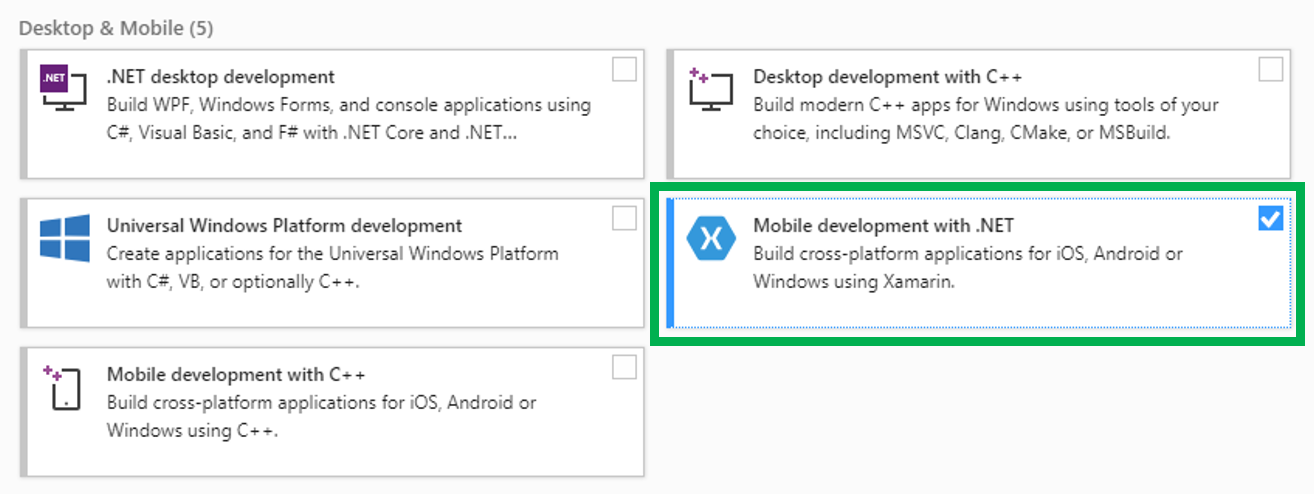
\includegraphics[width=0.7\linewidth]{images/auswahl_rahmenwerk/installation.png}    
    \caption{Auswahl des Xamarin-Rahmenwerks bei der Installation}
\end{figure}
Keine weiteren Einstellungen oder Auswahlen sind zwingend erforderlich, allerdings empfielt es sich noch zusätzlich das ".NET desktop development"-Paket installiert. Mit diesem kann man neue Technologien des .NET Frameworks in einer einfacheren Konsolenanwendung ausprobieren und kennenlernen.
\begin{figure}[H]
    \centering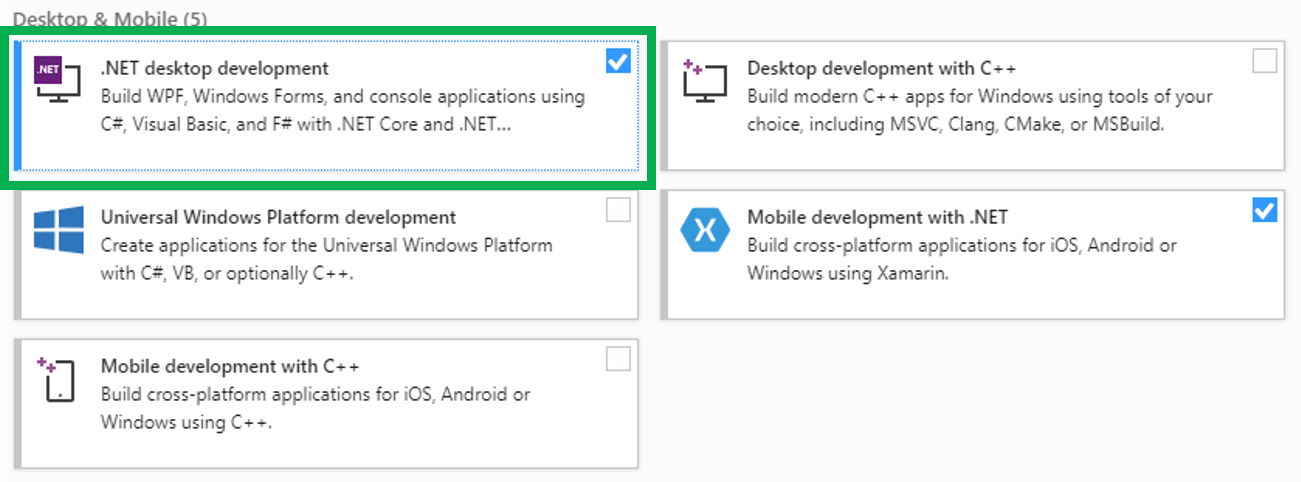
\includegraphics[width=0.7\linewidth]{images/auswahl_rahmenwerk/installation2.png}    
    \caption{Zusatzpaket für Desktop-Entwicklung mit .NET}
\end{figure}
Nach Fertigstellung der Installation von Visual Studio 2019 erscheint dieses am Desktop und im Startmeü als neues Icon. Zusätzlich zum Xamarin-Rahemnwerk sind die notwendigen Android-SDK-Komponenten auszuwählen und zu installieren. Diese sind notwendig ...

Nach dem Start von Visual Studio muss eine neue "Solution" angelegt werden. Diese beinhaltet alle Programmteile, welche für die Xamarin-Entwicklung benötigt werden. 

\begin{figure}[H]
    \centering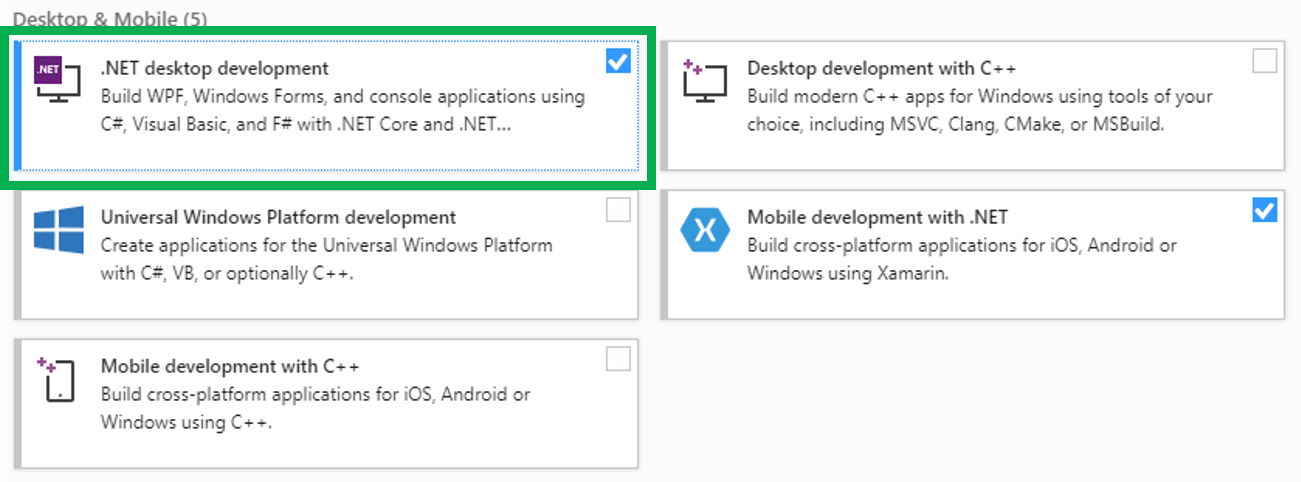
\includegraphics[width=0.7\linewidth]{images/auswahl_rahmenwerk/installation2.png}    
    \caption{Anlegen einer neuen Solution}
\end{figure}

\begin{figure}[H]
    \centering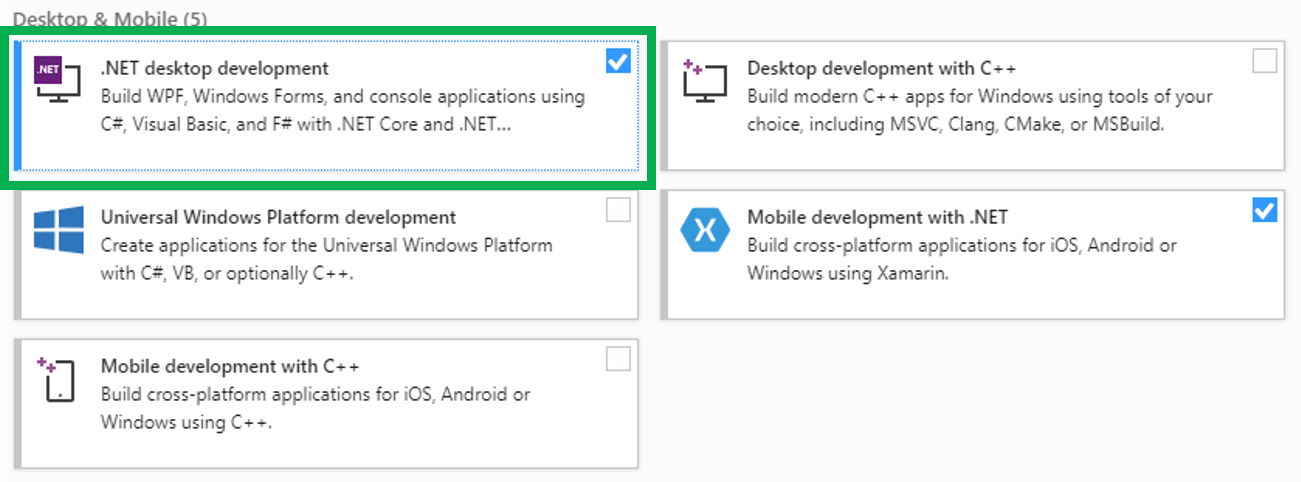
\includegraphics[width=0.7\linewidth]{images/auswahl_rahmenwerk/installation2.png}    
    \caption{Auswahl der beötigten Android Platformen}
\end{figure}
\begin{figure}[H]
    \centering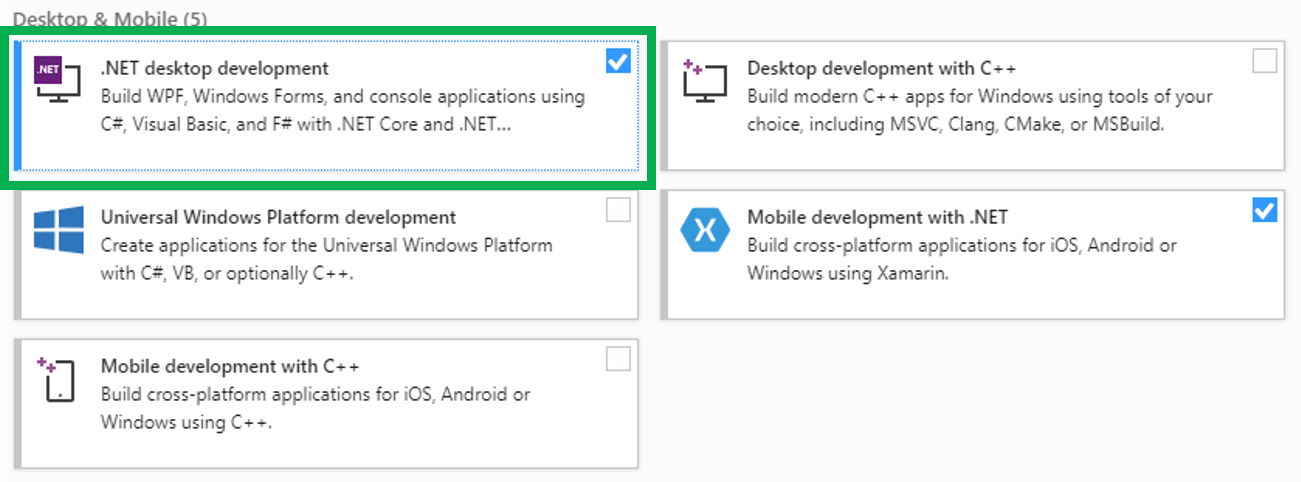
\includegraphics[width=0.7\linewidth]{images/auswahl_rahmenwerk/installation2.png}    
    \caption{Auswahl der benötigten Android Tools}
\end{figure}
%Android SDK komponente



%Weg vom Programm zur binary


\section{Gedanken}
% Als Programmiersprache wird in diesem Projekt die Sprache C verwendet. Die
% Programmentwicklung in C ist im Vergleich zur Entwicklung in der Assemblersprache schneller und einfacher möglich. Trotzdem bietet die Sprache C die
% Möglichkeit eines sehr hardwarenahen Zugriffs auf die verfügbare Peripherie des
% Controllers durch Zugriffsmöglichkeit auf die einzelnen Register.
% 
% Ziel der Build-Werkzeuge ist es somit, den C-Programmcode in Maschinencode
% zu übersetzen und diesen in das Intel-Hex-Format überzuführen.
% Zur Bewältigung dieser Aufgabe kann unter Windows entweder auf die offizielle Entwicklungsumgebung Atmel-Studio zurückgegriffen werden (vgl. Atmel Studio 7 2016) oder es wird das WinAVR-Softwarepaket verwendet, das eine wesentlich schlankere Installation bietet und einen Editor, den GCC-Compiler und
% alle weiteren benötigten Programme zur Erstellung des Hex-Files aus dem CProgrammcode mitliefert (vgl. Homepage WinAVR 2016). Das Programm kann
% von der Website direkt als Installer-Datei heruntergeladen werden.
% WinAVR liefert das Programm Programmer’s Notepad mit, das bereits alle benö-
% tigten Makros zur Übersetzung des Programms besitzt. Es reicht, eine beliebige
% Datei aus dem Ordner der Mikrocontrollersoftware mit Programmer’s Notepad zu
% öffnen und in der Menüleiste unter Tools die Auswahl Make all anzuklicken. Im
% Ordner wird eine Datei namens main.hex erzeugt, die nun beispielsweise mithilfe
% der Software des Programmieradapters zum Mikrocontroller übertragen werden
% kann.
% Unter Linux existieren bei den meisten Distributionen vorgefertigte Pakete unter
% dem Namen avr-gcc bzw. gcc-avr, welche die benötigte Software beinhalten. Sollte das Paket avr-libc nicht automatisch mitinstalliert werden, muss es manuell
% installiert werden. Zur Übersetzung des Projekts kann in der Kommandozeile in
% den Ordner mit den Quelldateien gewechselt und dort der Befehl make all ausgeführt werden. Der Befehl make clean löscht alle erzeugten Dateien, sodass nur
% mehr die Quelldateien übrigbleiben und make program überträgt das Programm
% zum Mikrocontroller. Zur Übertragung ruft make die Software avrdude auf, die
% eine Vielzahl verschiedener Programmiergeräte unterstützt. Um das verwendete
% Programmiergerät einzustellen, müssen in der Datei Makefile im Ordner mit den
% Quelldateien die Optionen AVRDUDE_PROGRAMMER und AVRDUDE_PORT abgeändert
% werden. Die Dokumentation des Programms avrdude liefert weitere Informationen
% über die unterstützten Programmer (vgl. AVRDUDE Documentation 2016).
% Achtung Der Mikrocontroller im Projekt wird mit einer Betriebsspannung von
% 3 V anstatt mit 5 V versorgt. Viele Programmer gehen jedoch davon aus, dass
% der Mikrocontroller mit 5 V betrieben wird. Vor dem Programmiervorgang sollte
% der Programmer auf 3 V-Betrieb umgestellt werden. Die genaue Vorgehensweise dazu muss der jeweiligen Dokumentation des Programmiergeräts entnommen
% werden.
% Fusebits Einige Grundfunktionen des Mikrocontrollers können über die sogenannten Fusebits eingestellt werden. Diese Bits werden, anders als die Konfigu-
% 1057. Auswahl Mikrocontroller
% rationsbits in gewöhnlichen Registern, nicht durch die Software am Controller,
% sondern direkt mithilfe des Programmieradapters eingestellt (vgl. ATmega 644
% Microcontroller Datasheet 2012, Seite 285 ff.). Für dieses Projekt müssen die Fusebits zur Einstellung der Taktquelle (CKSEL3..0) auf den Wert 0b1101 gestellt
% werden. Diese Einstellung steht für einen Low power crystal oscillator mit einer
% Frequenz zwischen 3 und 8 MHz. Außerdem ist es wichtig, das JTAG-Interface
% mithilfe des Bits JTAGEN (→ auf 0 setzen) zu deaktivieren, da die entsprechenden Pins des JTAG-Interfaces, das zum Debuggen verwendet werden kann, für
% andere Aufgaben benötigt werden. Möchte man die Mikrocontrollersoftware testen, bietet es sich an, das Bit EESAVE auf 0 zu setzen. Dadurch wird der Inhalt
% des EEPROMs nicht bei jedem Programmiervorgang gelöscht. So gehen die Einstellungen der Software nicht jedes Mal verloren, wenn ein Fehler in der Software
% ausgebessert wird.
% Zur Programmierung der Fusebits kann meist die entsprechende Software des
% Programmieradapters verwendet werden. Das Atmel-Studio und avrdude bieten
% die Funktionalität ebenfalls. Für avrdude bietet sich als komfortableres Frontend
% beispielsweise das Programm avr8-burn-o-mat an, das für alle gängigen Betriebssysteme auf der Projektwebsite heruntergeladen werden kann (vgl. AVR8 BurnO-Mat - a GUI for avrdude 2016).
% Wichtig Atmel bezeichnet Fusebits als programmed, wenn sie auf 0 gesetzt und
% als unprogrammed, wenn sie auf 1 gesetzt sind. Viele Programme zum Einstellen
% der Fusebits bieten eine Checkbox für die Einstellung an, die angehakt werden
% muss, um das Bit auf 0 zu setzen. Das kann verwirrend sein. In diesem Fall ist
% Vorsicht geboten. Die Dokumentation der entsprechenden Software sollte konsultiert werden, da eine falsche Einstellung der Taktquelle dazu führen kann, dass der
% Controller nicht mehr reagiert und zur „Wiederbelebung“ ein Taktsignal mittels
% Funktionsgenerator eingespeist werden muss.

%microsoft VS2019
%frei zugänglich
%nur auf windows, kein linux-support
%...